\documentclass[]{elsarticle} %review=doublespace preprint=single 5p=2 column
%%% Begin My package additions %%%%%%%%%%%%%%%%%%%
\usepackage[hyphens]{url}
\usepackage{lineno} % add
\providecommand{\tightlist}{%
  \setlength{\itemsep}{0pt}\setlength{\parskip}{0pt}}

\bibliographystyle{elsarticle-harv}
\biboptions{sort&compress} % For natbib
\usepackage{graphicx}
\usepackage{booktabs} % book-quality tables
%% Redefines the elsarticle footer
%\makeatletter
%\def\ps@pprintTitle{%
% \let\@oddhead\@empty
% \let\@evenhead\@empty
% \def\@oddfoot{\it \hfill\today}%
% \let\@evenfoot\@oddfoot}
%\makeatother

% A modified page layout
\textwidth 6.75in
\oddsidemargin -0.15in
\evensidemargin -0.15in
\textheight 9in
\topmargin -0.5in
%%%%%%%%%%%%%%%% end my additions to header

\usepackage[T1]{fontenc}
\usepackage{lmodern}
\usepackage{amssymb,amsmath}
\usepackage{ifxetex,ifluatex}
\usepackage{fixltx2e} % provides \textsubscript
% use upquote if available, for straight quotes in verbatim environments
\IfFileExists{upquote.sty}{\usepackage{upquote}}{}
\ifnum 0\ifxetex 1\fi\ifluatex 1\fi=0 % if pdftex
  \usepackage[utf8]{inputenc}
\else % if luatex or xelatex
  \usepackage{fontspec}
  \ifxetex
    \usepackage{xltxtra,xunicode}
  \fi
  \defaultfontfeatures{Mapping=tex-text,Scale=MatchLowercase}
  \newcommand{\euro}{€}
\fi
% use microtype if available
\IfFileExists{microtype.sty}{\usepackage{microtype}}{}
\usepackage{longtable}
\usepackage{graphicx}
% We will generate all images so they have a width \maxwidth. This means
% that they will get their normal width if they fit onto the page, but
% are scaled down if they would overflow the margins.
\makeatletter
\def\maxwidth{\ifdim\Gin@nat@width>\linewidth\linewidth
\else\Gin@nat@width\fi}
\makeatother
\let\Oldincludegraphics\includegraphics
\renewcommand{\includegraphics}[1]{\Oldincludegraphics[width=\maxwidth]{#1}}
\ifxetex
  \usepackage[setpagesize=false, % page size defined by xetex
              unicode=false, % unicode breaks when used with xetex
              xetex]{hyperref}
\else
  \usepackage[unicode=true]{hyperref}
\fi
\hypersetup{breaklinks=true,
            bookmarks=true,
            pdfauthor={},
            pdftitle={Have coaches changed how they select which players to give more minutes to?},
            colorlinks=true,
            urlcolor=blue,
            linkcolor=magenta,
            pdfborder={0 0 0}}
\urlstyle{same}  % don't use monospace font for urls
\setlength{\parindent}{0pt}
\setlength{\parskip}{6pt plus 2pt minus 1pt}
\setlength{\emergencystretch}{3em}  % prevent overfull lines
\setcounter{secnumdepth}{0}
% Pandoc toggle for numbering sections (defaults to be off)
\setcounter{secnumdepth}{0}
% Pandoc header


\usepackage[nomarkers]{endfloat}

\begin{document}
\begin{frontmatter}

  \title{Have coaches changed how they select which players to give more minutes
to?}
    \author[Pontificia Universidad Catolica de Chile]{Derek Corcoran\corref{c1}}
   \ead{derek.corcoran.barrios@gmail.com} 
   \cortext[c1]{Corresponding Author}
    \author[The University of Mississippi]{Nicholas M. Watanabe}
   \ead{nmwatana@olemiss.edu} 
  
      \address[Some Institute of Technology]{Department, Street, City, State, Zip}
    \address[Another University]{Department, Street, City, State, Zip}
  
  \begin{abstract}
  Since the NBA adopted the three point line in .
  
  It consists of two paragraphs.
  \end{abstract}
  
 \end{frontmatter}

\emph{Text based on elsarticle sample manuscript, see
\url{http://www.elsevier.com/author-schemas/latex-instructions\#elsarticle}}

\section{The Elsevier article class}\label{the-elsevier-article-class}

\paragraph{Installation}\label{installation}

If the document class \emph{elsarticle} is not available on your
computer, you can download and install the system package
\emph{texlive-publishers} (Linux) or install the LaTeX~package
\emph{elsarticle} using the package manager of your TeX~installation,
which is typically TeX~Live or MikTeX.

\paragraph{Usage}\label{usage}

Once the package is properly installed, you can use the document class
\emph{elsarticle} to create a manuscript. Please make sure that your
manuscript follows the guidelines in the Guide for Authors of the
relevant journal. It is not necessary to typeset your manuscript in
exactly the same way as an article, unless you are submitting to a
camera-ready copy (CRC) journal.

\subsection{Methods}\label{methods}

The basketball reference player season finder was used to extract the
per 100 team possessions stats, single season, during the three point
era (since season 1979-80), during the regular season (``Player Season
Finder Basketball-Reference.com'' 2017), and that information was
coupled twith the minutes per game played by each player, again
extracted from the basketball regerence player season finder but now in
the per game stats. We divided that dataset into 37 datasets, one for
each season from the 1979-80 season to the 2015-16 season.

For each season, the per 100 team possesion stats was used to fit a
global glm model (Nelder and Baker 1972) that explains the minutes per
game of each player based on the following variables: Two point shot
attempts per 100 possessions, two point shot percentage, three point
shots attempts per 100 possessions, three point shot percentage, free
thow attempts per 100 possessions, free throw percentage, total rebounds
per 100 possessions, assists per 100 possessions, steals per 100
possessions, blocks per 100 possessions, turnovers per 100 possessions,
points per 100 possessions and effective field goal percentage.

In order to be able to compare the strength of relationship of every
variable on the same scale, all of them were scaled and centered (Bro
and Smilde 2003) using the caret package (Kuhn and Johnson 2013).

For each season, we tested variables for collinearity. Then we fitted
every possible first order model not allowing models to coexist if they
had a pearosn correlation coefficient equal or higher than 0.7 (Dormann
et al. 2013). Then the models were ranked based on Akaike's Information
Criteria for small sample sizes (AICc) (Cavanaugh 1997) using the MuMin
Package (Barto{ń} 2013; Burnham and Anderson 2002). We didn't use model
averaging since even though collinear variables were prohibited to
coexist in the same model, these might coexist in the average model
(Cade 2015), thus we selected the best possible model for each season
selecting by AICc (Burnham and Anderson 2002). All of the analyses using
R statistical Software (Team 2016),

\subsection{Results}\label{results}

\begin{longtable}[c]{@{}rr@{}}
\toprule
Season & number of players\tabularnewline
\midrule
\endhead
1980 & 137\tabularnewline
1981 & 149\tabularnewline
1982 & 147\tabularnewline
1983 & 144\tabularnewline
1984 & 152\tabularnewline
1985 & 149\tabularnewline
1986 & 151\tabularnewline
1987 & 136\tabularnewline
1988 & 145\tabularnewline
1989 & 146\tabularnewline
1990 & 165\tabularnewline
1991 & 161\tabularnewline
1992 & 166\tabularnewline
1993 & 164\tabularnewline
1994 & 164\tabularnewline
1995 & 156\tabularnewline
1996 & 164\tabularnewline
1997 & 157\tabularnewline
1998 & 162\tabularnewline
1999 & 143\tabularnewline
2000 & 176\tabularnewline
2001 & 155\tabularnewline
2002 & 159\tabularnewline
2003 & 159\tabularnewline
2004 & 166\tabularnewline
2005 & 161\tabularnewline
2006 & 153\tabularnewline
2007 & 171\tabularnewline
2008 & 181\tabularnewline
2009 & 174\tabularnewline
2010 & 177\tabularnewline
2011 & 171\tabularnewline
2012 & 146\tabularnewline
2013 & 168\tabularnewline
2014 & 200\tabularnewline
2015 & 210\tabularnewline
2016 & 200\tabularnewline
\bottomrule
\end{longtable}

As we can see in figure 1, the AST is the variable that appears in most
season being selected in 36 of 37 seasons, followed by PTS and TRB being
selected in 29 and 25 seasons respectibely

\begin{figure}[htbp]
\centering
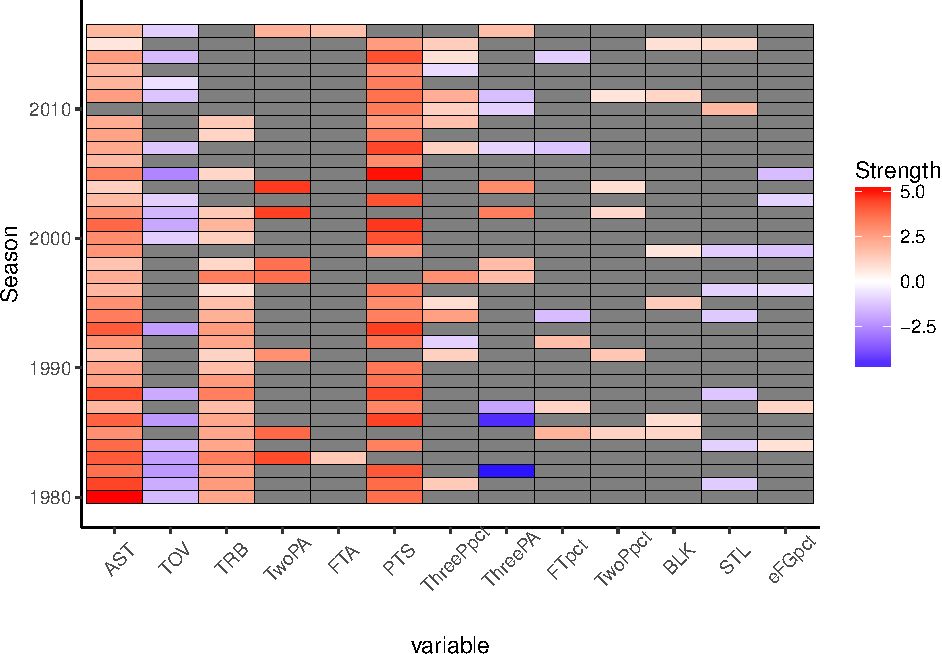
\includegraphics{Coaching_Selection_files/figure-latex/unnamed-chunk-5-1.pdf}
\caption{Strength of relationship by season}
\end{figure}

\begin{figure}[htbp]
\centering
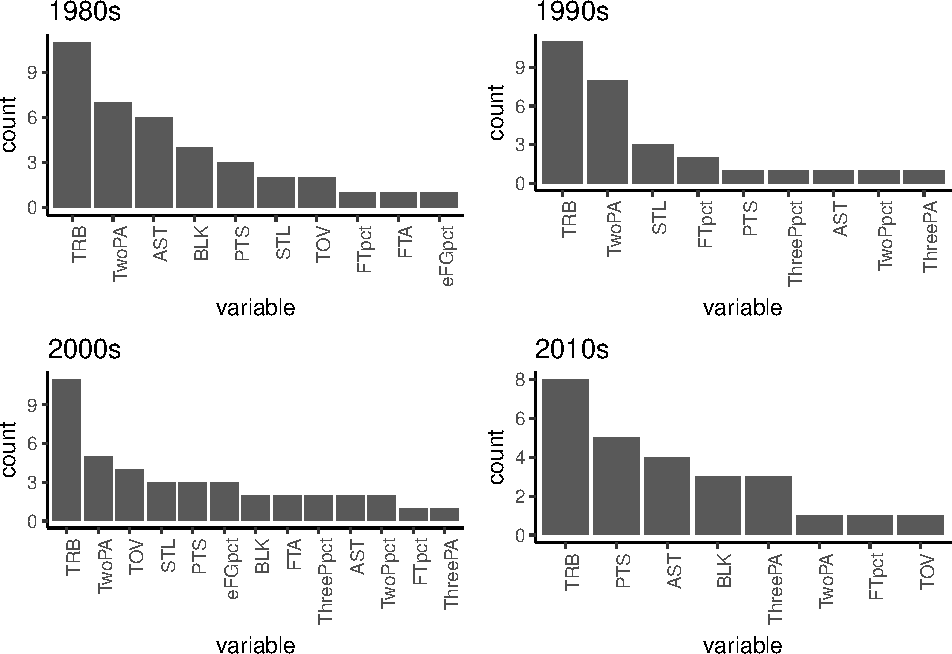
\includegraphics{Coaching_Selection_files/figure-latex/unnamed-chunk-6-1.pdf}
\caption{Strength of relationship by season for assists, Rebounds and
points}
\end{figure}

\paragraph{Functionality}\label{functionality}

The Elsevier article class is based on the standard article class and
supports almost all of the functionality of that class. In addition, it
features commands and options to format the

\begin{itemize}
\item
  document style
\item
  baselineskip
\item
  front matter
\item
  keywords and MSC codes
\item
  theorems, definitions and proofs
\item
  lables of enumerations
\item
  citation style and labeling.
\end{itemize}

\section{Front matter}\label{front-matter}

The author names and affiliations could be formatted in two ways:

\begin{enumerate}
\def\labelenumi{(\arabic{enumi})}
\item
  Group the authors per affiliation.
\item
  Use footnotes to indicate the affiliations.
\end{enumerate}

See the front matter of this document for examples. You are recommended
to conform your choice to the journal you are submitting to.

\section{Bibliography styles}\label{bibliography-styles}

There are various bibliography styles available. You can select the
style of your choice in the preamble of this document. These styles are
Elsevier styles based on standard styles like Harvard and Vancouver.
Please use BibTeX~to generate your bibliography and include DOIs
whenever available.

Here are two sample references: Barto{ń} (2013; Cade 2015).

\section*{References}\label{references}
\addcontentsline{toc}{section}{References}

Barto{ń}, Kamil. 2013. ``MuMIn: Multi-Model Inference. R Package Version
1.9. 13.'' \emph{The Comprehensive R Archive Network (CRAN), Vienna,
Austria}.

Bro, Rasmus, and Age K Smilde. 2003. ``Centering and Scaling in
Component Analysis.'' \emph{Journal of Chemometrics} 17 (1). Wiley
Online Library: 16--33.

Burnham, KP, and DR Anderson. 2002. ``Information and Likelihood Theory:
A Basis for Model Selection and Inference.'' \emph{Model Selection and
Multimodel Inference: A Practical Information-Theoretic Approach} 2.
Springer-Verlag New York: 49--97.

Cade, Brian S. 2015. ``Model Averaging and Muddled Multimodel
Inferences.'' \emph{Ecology} 96 (9). Wiley Online Library: 2370--82.

Cavanaugh, Joseph E. 1997. ``Unifying the Derivations for the Akaike and
Corrected Akaike Information Criteria.'' \emph{Statistics \& Probability
Letters} 33 (2). Elsevier: 201--8.

Dormann, Carsten F, Jane Elith, Sven Bacher, Carsten Buchmann, Gudrun
Carl, Gabriel Carr{é}, Jaime R Garc{í}a Marqu{é}z, et al. 2013.
``Collinearity: A Review of Methods to Deal with It and a Simulation
Study Evaluating Their Performance.'' \emph{Ecography} 36 (1). Wiley
Online Library: 27--46.

Kuhn, Max, and Kjell Johnson. 2013. \emph{Applied Predictive Modeling}.
Vol. 26. Springer.

Nelder, John A, and R Jacob Baker. 1972. ``Generalized Linear Models.''
\emph{Encyclopedia of Statistical Sciences}. Wiley Online Library.

``Player Season Finder Basketball-Reference.com.'' 2017. Accessed
February 27.
\url{http://www.basketball-reference.com/play-index/psl_finder.cgi}.

Team, R Core. 2016. ``R: A Language and Environment for Statistical
Computing. R Development Core Team, Vienna.''

\end{document}


